% !TeX spellcheck = en_US
\chapter{Introduction}
\label{chap:intro}

Wind energy is widely becoming recognized as one of the most cost efficient renewable energy sources.
It is predicted that by the end of 2014 the worlds wind energy production will reach 360GW which is around 4\% of the worlds electricity demand~\cite{worldwidewindcapacity}.
Heavyweight energy consumer USA has declared a goal of reaching 20\% wind energy of the total energy consumed in 2030~\cite{20percentenergy}, the European Union has committed to a similar goal that 20\% of the total energy consumption must come from renewable sources by 2020~\cite{directive2009}. For comparison, up to a 100\% of the total energy consumption of Denmark can be covered by wind power on days with optimal wind conditions~\cite{100percentwindenergy}.

Siemens Wind Power is one of the worlds leading producers of wind turbines, with a global market share of 9.5\% in 2012~\cite{worldmarketupdate2012}.
Siemens Wind Power is increasingly focusing on the offshore wind farm market.
The current setup of a wind farm requires additional infrastructure for management and control of the wind farm.
In addition to the wind turbines, a wind farm at Siemens Wind Power consists of multiple park regulators for turbine control, and a Supervisory Control And Data Acquisition (SCADA) system, which handles data aggregation, data logging and external network requests.

The SCADA system and park regulators does not scale automatically with the number of turbines. A park regulator can only handle power regulation for a certain amount of turbines, meaning the larger the wind farm, the more park regulators needs to be present to handle power regulation.
The power regulation performed by each park regulator, calculates if the power production of the wind farm is correct and adjusts and distributes the production goals of each turbine accordingly. This power regulation is, amongst others, based on the current state of each turbine connected to the park regulator. So in order to perform park regulations, the park regulator must first acquire the current state of each connected turbine.
% amongst others, based on the current state of each turbine connected to the park regulator.
%So in order to perform park regulations, the park regulator must first request the current state of each connected turbine. %in order to be able to calculate if the power production of the wind farm is correct.
%If the power production of the wind farm needs adjustment, the park regulator calculates new power production goals for each connected turbine and distributes these.

Increasing the number of turbines connected to a park regulator increases the number of turbine states that needs to be acquired, the number of power production goals that needs to be calculated and the number of these goals that needs to be distributed. Thus increasing the number of turbines connected to a park regulator, increases the time it takes to perform these regulations. The increase in power regulation time is primarily caused by the acquiring of states, since the park regulator must request an extra turbine state and wait for the corresponding reply per extra turbine added.
% will increase the time needed to collect the states of the connected turbines, calculate new power production goals and distribute these new power production goals to the connected turbines.
%Thus, increasing the number of turbines connected to a park regulator will increase the power regulation time.
%The increase in power regulation time is primarily caused by acquiring states of each turbine, since acquiring states involves . This  the fact that the park regulator must request a state from an extra turbine sand wait for the turbine to provide the state.

The linear relation between number of turbines and the power regulation time forces Siemens Wind Power to limit the number of turbines connected to a single park regulator. It also limits the scalability of the wind farm as adding more turbines may simultaneously require the addition of extra park regulators.

%Keeping the power regulation time low will allow for faster power regulation of the wind farm, which in turn will enable the wind farm to comply with the needs of the power grid faster. Faster compliance to the needs of the power grid will enable the wind farm to help in stabilizing the power grid faster, should power demand rise or fall unexpectedly. Thus, keeping a low power regulation time is important for a wind farm to be an asset of the power grid instead of a liability.

%If the power regulation time exceeds a certain threshold the wind farm is no longer able to satisfy the regulation demands required by the power grid.
%Thus, the number of turbines connected to a park regulator must be limited in order to uphold a power regulation cycle time that satisfy the requirements imposed by the power grid.

%It is desirable to have the turbines regulate and match the power grid's current need as fast as possible. According to Siemens Wind Power most of the delay for this regulation is because of the way regulation currently uses network traffic. Reducing the number of network transmission required to regulate a turbine is needed.
%The main problem being that with a centralized control systems a bottle neck is introduced through which all traffic must pass. This means the turbines must wait for the centralized control system to calculate and communicate values like the amount of power a single turbine must produce in order to meet the power production requirements of the entire wind farm.
%As the wind farm is expected to operate as a single unit the power production of a single turbine is affected by the power production of all other turbines.
%This interdependence between turbines forces the central control system to collect data from all turbines before a single new power production value can be calculated, which is time consuming. Adding turbines will additionally increase the time the centralized control system needs to calculate new power production values.
%To uphold a constant power production level for the entire wind farm near real-time control and regulation is necessary thus the time consumption of the centralized control system must be minimized in effect limiting the number of turbines the centralized control system is able to handle.

Both the park regulators and the SCADA system are essential for a Siemens Wind Power wind farm to function. Communication within the wind farm pass through these two components, and system failure in either the SCADA system or one of the park regulators may render parts of the wind farm unavailable, thus resulting in decreased control of the wind farm. This makes these components potential single points of failures to the wind farm. 

%Despite the fact that the wind farms has grown to a size that is becoming increasingly hard to manage as a centralized control system, little research has been done in the area of decentralization a wind farm managements and controls components.

As wind energy is recognized as one of the solutions to the renewable energy problem, wind park size and capacity keeps increasing.
The need for wind farm scalability and availability is thus not only a challenge for Siemens Wind Power but for the entire industry.

\section{Siemens Wind Power case}

% Beskriv topologi
% Regulerings algoritmen tager kun 30 ms. 150 ms er cycle time

\label{sec:SiemensCase}
Siemens Wind Power builds wind farms of different sizes, ranging from a single turbine to well above one hundred turbines \cite{simensOffShoreProjects, simensOnShoreProjects}. 

The current wind farm setup is illustrated on \cref{fig:currentSiemensSetup}. Today every turbine in a wind farm at Siemens Wind Power are equipped with computers for the purpose of turbine regulation and data logging. Every turbine is connected to a Wind Power Supervisor, which is a central component that aggregates data, stores data and handles wind park communication with the outside world. At Siemens up to eight Park Pilots and one Wind Power Supervisor are present per wind farm.

\begin{figure}[!h]
	\centering
	\scalebox{0.7}{\tikzstyle{line} = [draw, -latex']

\begin{tikzpicture}
[
	start chain=going right,
	diagram item/.style={
		minimum width=40pt,
		on chain,
	},
	mill item/.style={
			minimum width=10pt,
			on chain
	},
	comment item/.style={
			inner sep=5pt,
			draw,
			dashed,
	}
]

\newcommand\millFigure{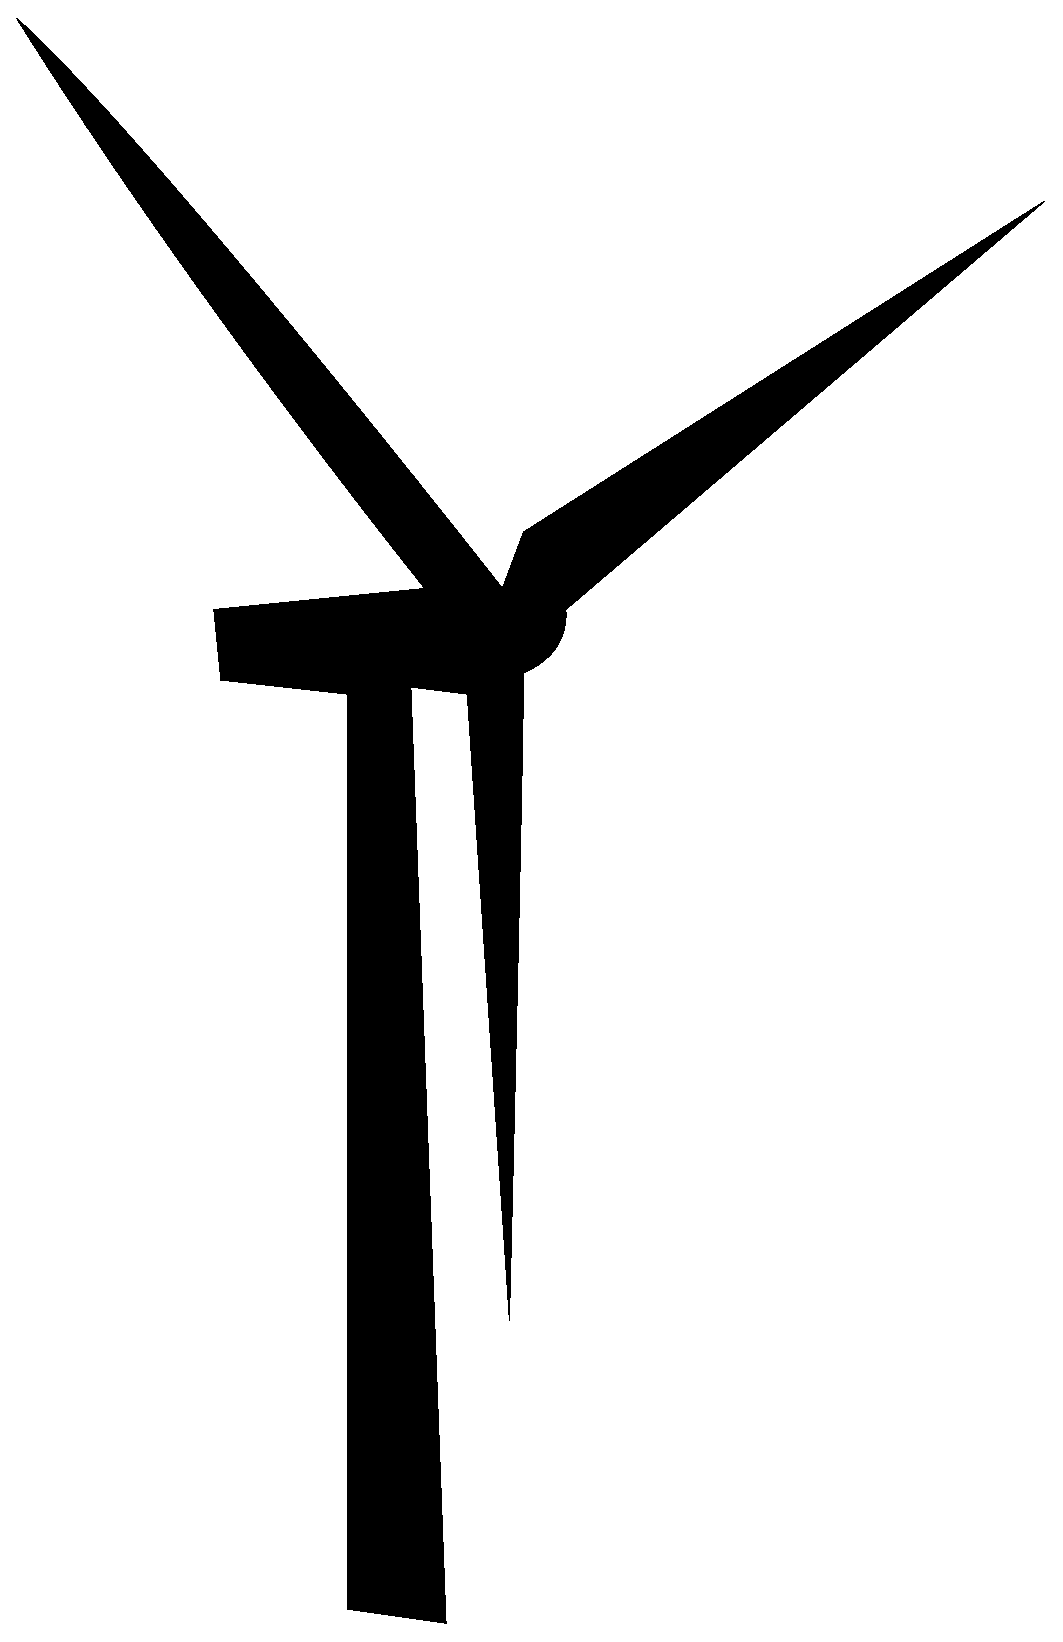
\includegraphics[width=0.7cm]{MillSiluet}}
\newcommand\multiMillFigure{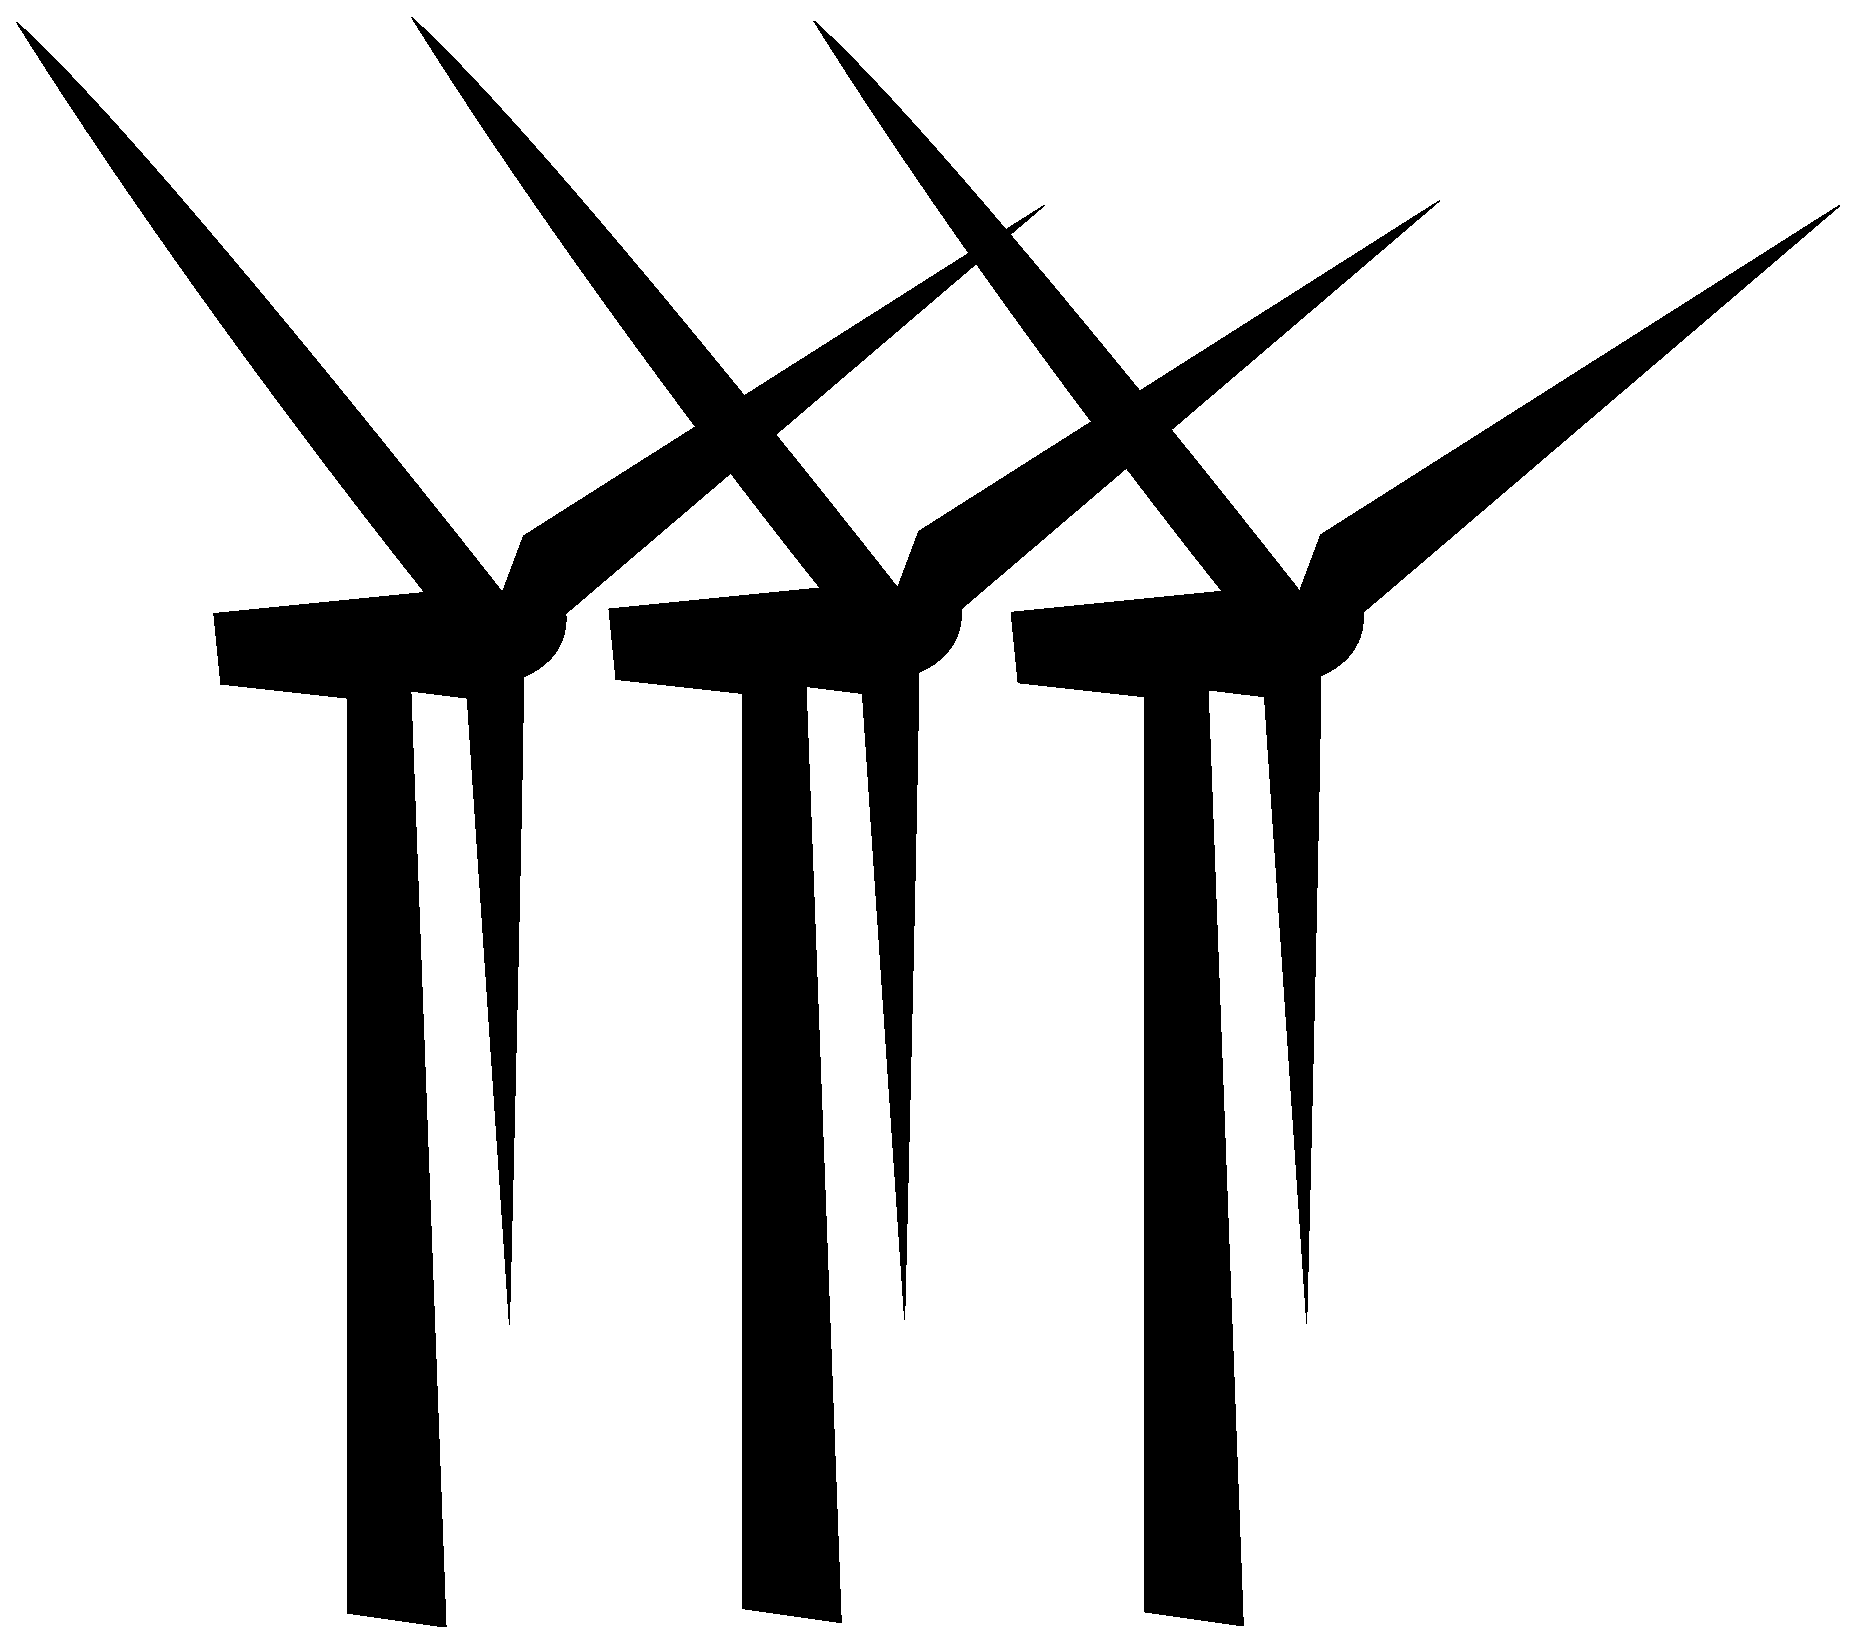
\includegraphics[width=4cm]{MultiMillSiluet}}

\begin{scope}[node distance=20mm and 10mm]

\node [
	diagram item,
	label=center:Internet
] (Internet) {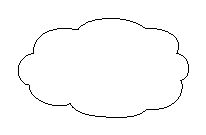
\includegraphics[width=4cm]{Cisco_BW/cloud}};

\node [
	continue chain=going below,
	diagram item,
	label={[label distance=0cm]80:Wind Power Supervisor}
] (wps){
\includegraphics[width=1.5cm]{Cisco_BW/fileserver}};

\node [
	start branch=1 going left,
	diagram item,
	label=above:High Performance Park Pilot
] (hppp){
\includegraphics[width=1.5cm]{Cisco_BW/fileserver}};

\node[
	comment item,
	align=left
](comment)[right=4cm of wps]{
	\begin{tabular}{l}
		\textbf{Wind Power Supervisor}  \\
		Control tasks\\
		- Noise control \\
		- Aviation light control \\
		Data \\
		- Aggregated historical \\
		- Reporting \\
		External communication \\
		- Network services \\
	\end{tabular}
};

\node [	
continue chain=going below,
mill item
] (millright){\multiMillFigure};

\node[
	comment item,
	align=left
](comment1)[right=3.0cm of millright]{
Each turbine contains logged \\
data with high resolution and \\
turbine control logic.};

\node [	
continue branch=1 going below,
mill item
] (millleft){\multiMillFigure};

\draw [->] (hppp.251) -- (millleft.101) node [near start, left] {1} node [midway] (hiddenNode){};

\node[
	comment item,
	align=left
](comment2)[left=1.7cm of hiddenNode]{
HPPP \\
getCurrentStatus() \\
calculateSetpoints() \\
setNewSetpoints() };

\path [line,dashed] (wps) -- (comment);
\path [line,dashed] (millright) -- (comment1);
\path [line,dashed] (hiddenNode) -- (comment2);

\draw [->] (hppp.280) -- (millleft.84) node [near end, right] {*};
\draw [<-] (hppp.265) -- (millleft.93);

\draw (Internet) -- (wps);
\draw (wps) -- (hppp) node [near start, above] {1} node [near end, below] {*};
\draw (wps) -- (millright) node [near start, left] {1} node [near end, right] {*};

\end{scope}

\end{tikzpicture}}
	\captionsetup{format=plain,font=footnotesize,labelfont={bf,defaultCapFont},labelsep=quad,singlelinecheck=no}
	\caption[The current Siemens wind farm system overview]{
		\label{fig:currentSiemensSetup} 
		\footnotesize{%
			The current Siemens system overview.
		}
	}
\end{figure}

For every transformer station in the wind farm there is a Park Pilot. The Park Pilots are responsible for wind farm regulation, meaning issuing production goals for each turbine, based on the how much power the entire wind farm should produce and the state of each turbine within the wind farm. A production goal is how much power a given turbine should produce and are from hereon called a \textit{setpoint}. The state of a turbine is information regarding how much power the turbine can produce, based on wind and weather conditions amongst others, and the amount of power the turbine currently is producing. 

The Park Pilots at Siemens Wind Power spends 150 ms performing a single regulation. Regulation is performed continuously, making regulation a cyclic process. The calculation of setpoints for each turbine consist of a number of steps as illustrated on \cref{fig:currentSiemensCycleTime}. First the Park Pilot must request the state of each turbine in order to calculate new setpoints. The Park Pilot must wait for each turbine to answer the request. After receiving data from each turbine new setpoints are calculated and distributed to the turbines. The buffer is added to make sure setpoints has been properly distributed and that individual turbines have time to adjust their power production according to the new setpoint before a new request for turbine data is sent. Also the time spent waiting for states may vary depending on the current traffic of the network as well as the response time of the individual turbines.

\begin{figure}[!h]
	\centering
	

{ %The brackets issolate the enviroment

\tikzstyle{line}		 	= [draw]

\makeatletter
\ifcsname c@wavenum\endcsname %Only create one counter
\else
	\newcounter{wavenum}
\fi
\makeatother

\newcommand*{\bitvector}[3]{
  \draw[fill=#3] (t_cur) -- ++( .1, .3) -- ++(#2-.2,0) -- ++(.1, -.3)
                         -- ++(-.1,-.3) -- ++(.2-#2,0) -- cycle;
  \path (t_cur) -- node[anchor=mid](textNode) {#1} ++(#2,0) node[time] (t_cur) {};
  }

% \known{val}{length}
\newcommand*{\known}[2]{
    \bitvector{#1}{#2}{white}
}

% \unknown{length}
\newcommand*{\unknown}[2]{
    \bitvector{#1}{#2}{black!20}
}

% \nextwave{name}
\newcommand{\nextwave}[1]{
  \path (0,\value{wavenum}) node[time] (t_cur) {};
  % \path (0,\value{wavenum}) node[left] {#1} node[time] (t_cur) {};
  \addtocounter{wavenum}{-1}
}

\newcommand{\timeSpanLabel}{
	\node (CycleTimeLabel) [rectangle, above right = 0.7cm and -2.7cm of textNode, inner sep=0pt] {~~~~~~~Regulation cycle time~~~~~~~};	  
}

\newcommand{\timeSpanA}{
	\node (t_timeSpanA) [point, above = 0 of t_cur] {};	  
}

\newcommand{\timeSpanB}{
	\node (t_timeSpanB) [point, above =0 of t_cur] {};

  \graph[use existing nodes]{
  	t_timeSpanA --[time span=1cm] CycleTimeLabel;
   	CycleTimeLabel.south --[time span=-0.24cm] t_timeSpanB;
  }; 
    	
}


%%% End of timing.sty
\begin{tikzpicture}[
	point/.style={inner sep=0pt}, %circle,minimum size=2pt,fill=red},
	draw=black, 
	yscale=.8,
	xscale=1,
	hv path/.style={to path={-| (\tikztotarget)}},
	vh path/.style={to path={|- (\tikztotarget)}},
	skip loop v/.style={to path={-- ++(#1,0) |- (\tikztotarget)}},		
	skip loop h/.style={to path={-- ++(0,#1) -| (\tikztotarget)}},
	time span/.style={to path={-- ++(0,#1) -| (\tikztotarget)}},
	graphs/every graph/.style={edges=rounded corners}	
	]
	
  \tikzstyle{time}=[coordinate]
  \setlength{\unitlength}{1cm}
  \setcounter{wavenum}{0}
    
  %\nextwave{Regulation Time} \unknown{SendData}{2} \known{WaitForData}{5} \unknown{ReciveData}{2} \unknown{Calculate}{2}\unknown{SendSP}{2}
  \nextwave{} \timeSpanA \unknown{Request states}{2.7} \known{Wait for states}{2.8} \unknown{Read states}{2.3} \timeSpanLabel \unknown{Calculate}{2}\unknown{Send setpoints}{3} \known{time buffer}{2} \timeSpanB
  
  
  
\end{tikzpicture}
}

	\captionsetup{format=plain,font=footnotesize,labelfont={bf,defaultCapFont},labelsep=quad,singlelinecheck=no}
	\caption[The current Siemens wind farm system overview]{
		\label{fig:currentSiemensCycleTime} 
		\footnotesize{%
			Park Pilot regulation cycle.
		}
	}
\end{figure}

Every turbine has a database for data logging purposes, this database is replicated to the Wind Power Supervisor.
The Wind Power Supervisor does data aggregation on data from each turbine as well as store a copy of the replicated data.
The turbines, Wind Power Supervisor and Park Pilots are connected with a gigabit network, which currently has plenty of extra capacity in terms of available bandwidth.
Internally, the turbine has more than 50 control points and 200 measurement points. The measurement points are sampled continually every 50 ms.

%\begin{figure}
%	\centering
%	\begin{sequencediagram} %Created using pgf-umlsd
%		\newthread{reg}{:Park Pilot}
%		\newinst[2]{turbine}{:Turbine}
%	
%		\begin{sdblock}{each turbine}{}
%			\mess[1]{reg}{getCurrentStatus}{turbine}
%			\mess[1]{turbine}{status}{reg}
%		\end{sdblock}
%		
%		\begin{call}{reg}{calculateAllSetpoints()}{reg}{}
%		\end{call}
%	
%		\begin{sdblock}{each turbine}{}
%			\mess[1]{reg}{setNewSetpoint}{turbine}
%		\end{sdblock}
%					
%	\end{sequencediagram}
%
%	\captionsetup{format=plain,font=footnotesize,labelfont={bf,defaultCapFont},labelsep=quad,singlelinecheck=no}
%	\caption[Regulator calculation sequence]{
%		\label{fig:dataComputationSequence} 
%		\footnotesize{%
%			Regulator calculation sequence.
%		}
%	}
%\end{figure}

\section{Thesis motivation}
\label{sec:ThesisMotivation}
Today's setup at Siemens Wind Power (\cref{sec:SiemensCase}) is an example of a system wished to be made decentralized. The current setup poses the following challenges to Siemens:  

\begin{itemize} 
	\item Single point of failure. Should a Wind Power Supervisor or a Park Pilot fail, a part of the wind farm will become unavailable.
	\item Low scalability. The Wind Power Supervisors and Park Pilots does not scale well with the number of turbines. This is reflected in the wind farm regulation performance. Today a wind farm regulation cycle time is 150 ms. This regulation cycle time is set after worst case setpoint retrieval time, worst case new setpoint calculations and worst case time it takes to broadcast new setpoints. This ultimately depends on worst case number of turbines per Park Pilot.
	\item High regulation cycle time. As mentioned, the regulation cycle time of the current Siemens system is 150 ms and is a direct result of the low scalability. Siemens expects a demand for a lower regulation cycle time in the future.
\end{itemize}

Siemens wishes to decentralize the Wind Power Supervisor and Park Pilots by distributing their functionality to the turbines, utilizing the free computing capacity of the computers already residing in every turbine. This would increase availability by lowering the possibility of single point of failure. Furthermore, this would increase scalability of the system, opening for performance optimizations of the wind farm regulation cycle time by decreasing the coupling between the regulation cycle time and the number of turbines per Park Pilot. 

\section{Problem statement}
\label{sec:problemStatement}

The purpose of this thesis is to design, implement and evaluate a solution for a Siemens Wind Power wind farm, where the Wind Power Supervisor and the Park Pilots are decentralized by utilizing the free computational capacity residing in every turbine for the Siemens Wind Power case. The proposed decentralized solution must maintain the ability to control the turbine's power production in order to reach the power production goal of the wind farm. 

\paragraph{Specifically, the following problems are addressed:}
\begin{description} % [label={\arabic*.}, ref=\textit{\arabic*}]
	%	\label{PS:Q:1}
	\labitem{Feasibility}{PS:Q:Feasibility} How can we best re-implement the current Siemens system (\cref{sec:SiemensCase}) as a system where the Wind Power Supervisor and the Park Pilots are decentralized?
	%	\label{PS:Q:4}
	\labitem{Availability}{PS:Q:Availability} Can we create a solution where removing one or more nodes from the system at runtime does not cause system failure?
	%	\label{PS:Q:3}
	\labitem{Performance}{PS:Q:Performance} Can we create a solution that scales such that the number of turbines does not impact the regulation cycle time?
	%	\item Can we, with the new decentralized solution, reduce the current regulation cycle time of 150 ms?
	%	\label{PS:Q:2}
	\labitem{Scalability}{PS:Q:Scalability} How will the new decentralized solution influence regulation time of a single regulations cycle compared to the current Siemens system?
	
%	\labitem{Scalability}{PS:Q:Scalability} How will the new decentralized solution influence the following parameters compared to the current Siemens system:
%	\begin{enumerate}
%		\item Time in milliseconds of a single regulation cycle.
%		\item Network traffic measured in bits per second.
%		\item Memory impact measured in bytes.
%	\end{enumerate}
\end{description}

The decentralized solution will be implemented as a prototype, for proof of concept and test purposes.

\section{Thesis scope}
\label{sec:thesisScope}
The scope of this thesis is limited to the following areas:

\begin{itemize}
	\item Analysis and identification of state of the art software components that will enable a reimplementation of the current Siemens system as a decentralized system to address the problem denoted as \ref{PS:Q:Feasibility}.
	\item Implementation of a decentralized solution that duplicates the central features of a Park Pilot needed to address problems \ref{PS:Q:Availability}, \ref{PS:Q:Performance} and \ref{PS:Q:Scalability} of the problem statement.
	\item Comparison of the decentralized solution to the current Siemens system to address problems \ref{PS:Q:Performance} and \ref{PS:Q:Scalability}.
\end{itemize}

The features of the Wind Power Supervisor will not be implemented in the decentralized solution.

\section{Related work}
The popularity of wind energy has lead to massive research within the area. Generally the research is focused on a number of areas:

\begin{itemize}
	\item Optimization of turbine design and construction materials.
	\item Turbine and wind farm control.
	\item Integration of wind farms into existing power grids.
	\item Wind flow prediction and simulation.
	\item Wake flow optimization and simulation.
	\item Offshore wind farms.
\end{itemize}

%\section{Decentralized systems}
%With the coming era of Internet of Things (IoT) the focus on decentralized systems and autonomic agents is greater than ever.
%IoT devices must be able to communicate with each other directly without the need for an intermediate central server.
%Furthermore the IoT devices must be largely autonomous since they cannot rely on a lasting connection to a server for control.
%
%A new approach to control of wind farms is to utilize game theory\cite{AModelFreeApproachToWindFarmControl}.
%The turbines in a farm must cooperate to reach the desired goal of a chosen output.
%The game theory approach use an iterative learning algorithm that converges against the optimal output after n iterations.

\subsection{Aeolus}
The Aeolus project was a large scale EU supported project which lasted from may 2008 to april 2011. It included project partners from 
Aalborg University, Industrial Systems and Control Ltd in Glasgow, University of Zagreb, Energy Research Centre of the Netherlands and Vestas Wind Systems A/S.
The main objectives of the project was to research and develop predictions of flows and incorporate data from a network of sensors, as well as research and develop control paradigms that acknowledges the uncertainty in the modeling and dynamically manages the flow resource in order to optimize specific control objectives.
The project is relevant to this thesis because several approaches to control of a wind farm was evaluated.

One approach was the hierarchical approach which uses local control on the turbine level and global control on the wind farm level~\cite{HeirarchicalWindFarmControl}.
Setpoints for the global output of the wind farm are received by the controller on the wind farm level.
So is the output for each turbine and the maximum available output for each turbine.
The global controller calculates setpoints for each turbine based on the global setpoint and each turbines current and possible output.
The controllers on turbine level is responsible for reaching the setpoint calculated by the global controller as well as making each turbine reach the setpoint in the most optimal manner(gearing, avoid ice over, avoid oscillation).
The hierarchical approach is similar to the current approach used in the Siemens case.

Another approach was the decentralized feed-forward approach~\cite{DecentralisedFeedforwardControlOfWindFarms} which takes advantage of the placement of turbines in a wind farm by letting upwind turbines feed wind data to downwind turbines. 
This allows downwind turbines to make adjustments to their production in order to exploit the coming wind in the best way.
Furthermore, a restricted communication model is used allowing turbines only to communicate with their neighbors.
Using this decentralized feed-forward approach to control a wind farm can help even out the output of the farm since downwind turbines has additional information regarding wind speed to come to act upon. If upwind turbines power production is also a part of the feed-forward package downwind turbines may also be able to regulate overall wind farm production by evening out spikes from upwind turbines.
In addition, by only communicating with neighboring turbines in order to achieve improvements in output the need for a centralized node is alleviated.

\subsection{Other related works}
The European Union has a number of sponsored projects beside the Aeolus project:
\begin{itemize}
	\item IRPWIND, which aim to accelerate the transition towards low-carbon energy through better integration of the European research activities~\cite{IRPWIND}. The program has six subprogrammes:
	\begin{enumerate}
		\item Wind conditions
		\item Aerodynamics
		\item Structures and Materials
		\item Wind Integration
		\item Offshore Wind Energy
		\item Research Infrastructure
	\end{enumerate}
	\item INNWIND, which focus is on accelerating the process of realizing the 20MW turbine~\cite{INNWIND}.
	\item EERA-DTOC, which focus is on creating a software tool for optimizing offshore wind farm design and clusters of wind farms~\cite{eera-dtoc}.
\end{itemize}

Likewise the  United States of America has a number of projects most of them performed by Sandia National Laboratories or National Renewable Energy Laboratory:
\begin{itemize}
	\item SWiFT, which focus is on wake effects, turbine control and rotor development~\cite{SWiFT}.
	\item Offshore Wind, which focus on large rotor development and simulation algorithms~\cite{offshoreWind}.
	\item Active Power Control, focus on using wind turbines for active control of the power grid~\cite{activePowerControl}.
\end{itemize}

The area of the supporting software architecture and software stack is not a topic that has received much attention, presumably because the prevailing solutions are proprietary and therefore not available for public research.
This thesis adds insight into which software components and technologies could be used in a wind farm, thus filling in some of the gap in the research area.

%\subsection{Game theory control}
%A new approach to control of wind farms is to utilize game theory\cite{AModelFreeApproachToWindFarmControl}.
%The turbines in a farm must cooperate to reach the desired goal of a chosen output current.
%The game theory approach use an iterative learning algorithm that converges against the optimal output after n iterations.
%According to the above referenced article improvements on up to 25\% is possible compared to other algorithms currently in use.

%\section{Enabling comparison of current Siemens system with decentralized solution}
%\todo{Bad title, move to another chapter}
%In order to address the problems presented in \cref{sec:problemStatement} a common ground must be established for comparison purposes. The decentralized solution proposed in this thesis will not be directly comparable to the current Siemens system because we are unable to duplicate the environment of the current Siemens system. As a consequence of this a centralized solution resembling the current Siemens system must be developed to enable a comparison. As presented in \cref{fig:projectDiffOverview} there exist a difference between the current Siemens system and the centralized solution as well as a difference between the centralized solution and the decentralized solution, illustrated by deltas.
%
%\begin{figure}[!h]
%	\centering
%	\begin{tikzpicture}[
	node distance = 0.3cm,
	auto,
	block/.style={draw, rectangle, text width=5em, text centered, minimum height=5cm}		
	]
% Place nodes
\node [block]			(Siemens)												[label=above:Siemens system]	{};
\node []					(SimCen)		[right = of Siemens] 	{$\Delta$};
\node [block]			(OurCent)		[right = of SimCen] 	[label=above:Centralized solution]	{};

\begin{scope}[on background layer]
\node [block] 		(Central) 	[fit=(Siemens) (OurCent), inner sep=20pt] {};
\node []					(CenDece)		[right = of Central] 	{$\Delta$};
\node [block]			(DeCent)		[right = of CenDece] 	[label=above:Decentralized solution] {};
\end{scope}

\end{tikzpicture}
%	\captionsetup{format=plain,font=footnotesize,labelfont={bf,defaultCapFont},labelsep=quad,singlelinecheck=no}
%	\caption[Comparison overview]{
%		\label{fig:projectDiffOverview} 
%		\footnotesize{%
%			Comparison overview.
%		}
%	}
%\end{figure}
%
%The delta between the current Siemens system and the centralized solution is minimized as much as possible based on information about the current Siemens system delivered by Siemens Wind Power. Since the operation and regulation of the current Siemens system is proprietary the full system information is not available. To make up for the missing information a number of assumptions has been done about the current Siemens system which is also a part of the delta. These assumptions will be detailed further in \cref{cha:existingSystem}. 
%
%The delta between the centralized solution and decentralized solution describes the difference in operation of a centralized system and a decentralized system.

%ASK SIEMENS HOW TO COMPARE AND MORE CONSTRAINTS??? 

%The purpose of this thesis is to design, implement and evaluate a distributed system solution for the Siemens Wind Power case. The solution must be able to provide the same features as the current solution. The goal of the new solution is to improve scalability, availability and performance by distributing the Park Pilot and the Wind Power Supervisor onto the turbines and thereby eliminate single point of failures and make performance scale with the amount of turbines within the wind farm. 

%To realize this the system must be redesigned as a distributed system. The solution must be able to handle external requests, communication between the nodes and distribution of data, according to the Siemens case. Furthermore the solution must have a single interface for control of, and interaction with, all the nodes, in order to maintain the illusion of the wind farm serving as a single system. This means ease of access must be maintained even though computation and data is distributed among nodes. Traffic must be routed to a turbine controllers with free capacity through a single interface, without external systems being aware of it.

%This roughly leaves three essential components: A component that handles distribution of data, a component that handles communication between nodes and a load balancer, to keep track of available resources on each node. The aim to investigate, analyze and evaluate state of the art technologies within each component area and choose the technologies best suited for the Siemens case. The technologies will be weighed in terms of features with regards to the Siemens case and performance.
%
%Furthermore we aim to develop a prototype, which runs the developed solution, for proof of concept purposes. The prototype will be compared to the existing Siemens solution with respect to performance, availability and redundancy. ASK SIEMENS HOW TO COMPARE AND MORE CONSTRAINTS??? 
%
%The Siemens case presents the following constraints to the project:
%\begin{itemize}
%	\item CPU power. Our solution must be able to run on a standard consumer hardware.
%	\item Network bandwidth. Siemens uses gigabit network.
%	\item Topology. Siemens wind farms uses ring and star topology.
%\end{itemize}



% % The below snippet might come handy later on % % %
% % % % % % % % % % % % % % % % % % % % % % % % % % %
%A distributed system is a network of hardware or software components, which communicates and coordinate their actions only by message passing\cite{coulouris2005distributed}, as illustrated on \cref{fig:distributedSystem}. Each component have their own local memory every component and interact with each other in order to achieve a common goal. The nodes can be physically close, connected via a local network, or geographically distant, connected by a wide area network. An important goal of a distributed system is location transparency\cite{coulouris2005distributed} to create the illusion of the entire system acting as a single computer even though it is comprised of several nodes. Examples of distributed systems vary from aircraft control systems to the Internet to massively multiplayer online games. 
% Er det bare mig eller er det lidt rigeligt at sige at systemet agere som en enkelt computer? Lad hellere sige noget om at opnå et fælles mål? Multiplayer spil er vel ikke distribuerede systemer, men mere server client systemer.

%\begin{figure}
%	\centering
%	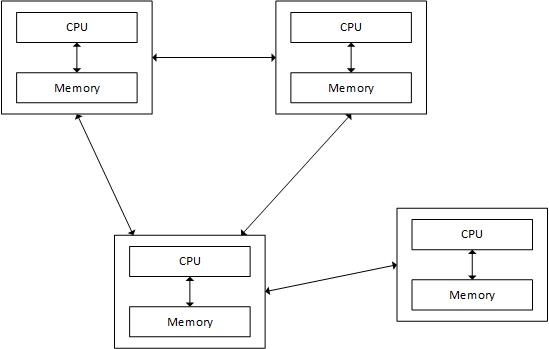
\includegraphics[width=0.7\textwidth,natwidth=510,natheight=542]{DistributedSystem.jpg} 
%	\captionsetup{format=plain,font=footnotesize,labelfont={bf,defaultCapFont},labelsep=quad,singlelinecheck=no}
%	\caption[Distributed Computing System with 2 nodes]{
%		\label{fig:distributedSystem} 
%		\footnotesize{%
%			A distributed system with 4 nodes.
%		}
%	}
%\end{figure}

%Distributed systems offer many benefits over centralized systems including the following\cite{IBM2005TXSeries}:
%\begin{itemize}
%	\item Scalability: It is easy to add nodes to the system, should the size of the system increase.
%	\item Redundancy: Several nodes can provide the same service, so if a node crashes, there are many to replace it. Additionally, from a cost perspective, each node does not have to be expensive, because many smaller nodes can be used as replacement.
%\end{itemize}
% Vi burde nok også snakke om ulemper? Og det er vel bare ting som er mulige at opnå?

